\documentclass[tikz]{standalone}
\usepackage{tikz}
\definecolor{bgdark}{HTML}{171D2B}
\definecolor{acc}{HTML}{F7B538}
\begin{document}
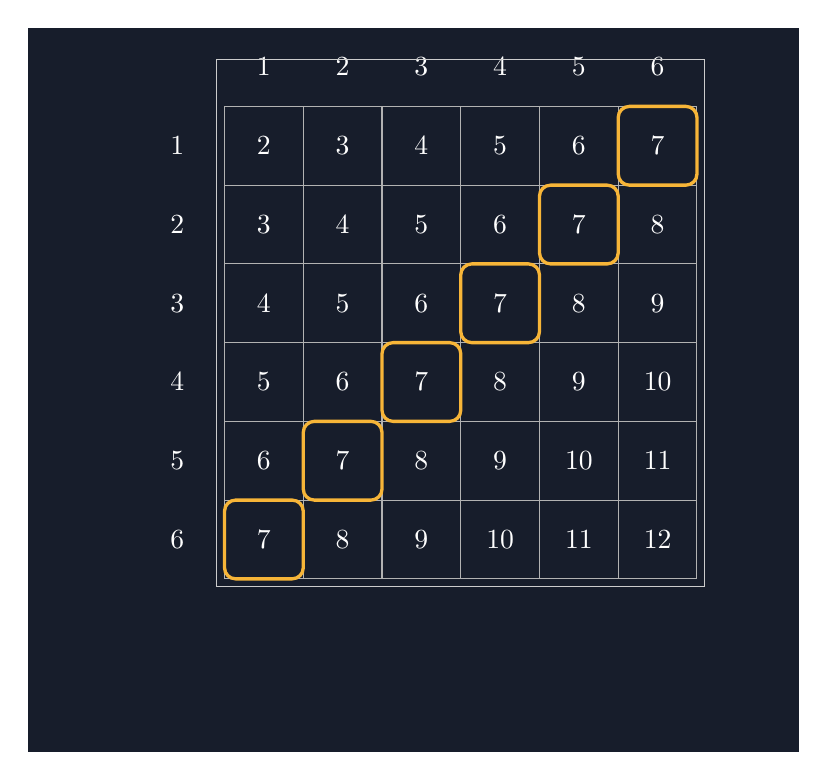
\begin{tikzpicture}[text=white, x=1.0cm, y=1.0cm]
\fill[bgdark] (-1.5,-1.2) rectangle (8.3,8.0);
\foreach \i in {1,...,6} {
  \node at (\i+0.5, 7.5) {\i};
  \node at (0.4, 7.5-\i) {\i};
}
\foreach \i in {1,...,6}
  \foreach \j in {1,...,6}
    \node at (\i+0.5, 7.5-\j) {\pgfmathtruncatemacro{\s}{\i+\j}\s};
\draw[gray!60] (1,1) grid (7,7);
\foreach \i in {1,...,6} {
  \pgfmathtruncatemacro{\j}{7-\i}
  \draw[acc, very thick, rounded corners] (\i, \i) rectangle (\i+1, \i+1);
}
\draw[gray!40] (0.9,0.9) rectangle (7.1,7.6);
\end{tikzpicture}
\end{document}
